\documentclass{beamer}
\usepackage[utf8]{inputenc}

\title{Inner Minkowski Dimension of Products of Fractal Strings}
\author{Joseph Ingenito, Peter Tonuzi }
\institute[]{The College of New Jersey}
\date{December 2020}
\logo{

\includegraphics[scale=0.10]{tcnj-logotype-400-200.jpg}
}
\subject{MAT 492, Spring 2020} % metadata
\usepackage{animate}
\usepackage{amsmath}
\usepackage{systeme}
\usepackage[dvipsnames]{xcolor}

\newcommand{\R}{\mathbb{R}}
\newcommand{\N}{\mathbb{N}}
\newcommand{\SL}{\mathcal{L}}
\newcommand{\SM}{\mathcal{M}}
\newcommand{\Om}{\Omega}
\newcommand{\W}{\mathcal{W}}
\DeclareMathAlphabet{\mathpzc}{OT1}{pzc}{m}{it}
\newcommand{\p}{\mathpzc{p}}
\newcommand{\q}{\mathpzc{q}}
\newcommand{\z}{\mathpzc{z}}

\begin{document}

\frame{\titlepage}

\begin{frame}
\frametitle{What is a Fractal String}

\begin{definition}
A {\bf fractal string} $\Om$ is a bounded open subset of the real line.
\end{definition}

\pause
\vspace{.2 in}

$\Omega = \displaystyle\bigcup_{j = 1}^\infty \ell_j$,\qquad $\displaystyle \SL = \text{Vol}_1\left(\Omega\right) = \sum_{j = 1}^\infty \ell_j \implies \lim_{j \to \infty} \ell_j = 0$.

\pause
\vspace{.2 in}

$\ell_1 \geq \ell_2 \geq \ell_3 \geq \cdots \geq 0$

\end{frame}

\begin{frame}{Inner-Tubular Neighborhood}

\begin{definition}
{\bf Inner-tubular neighborhood}:\quad $V(\epsilon) = \text{vol}_1\{x \in \Omega\ |\ d(x,\partial\Omega) < \epsilon\}$
\end{definition}

\pause
\vspace{.2 in}

{\bf Counting function}:$\displaystyle \quad N_{\Omega}(x) = \sum_{\ell_j \geq x}1$

\vspace{.2 in}

{\bf More Notation}: $\displaystyle \quad \W_\Om(x) = \sum_{j:\ell_j < x}{\ell_j}$

\vspace{.2 in}

$V(\epsilon) = 2\epsilon \cdot N_\Om\left(2\epsilon\right) + \W_\Om\left(2\epsilon\right)$

\end{frame}

\begin{frame}{Inner-Minkowski Dimension of a Fractal String}

\begin{definition}
{\bf Inner-Minkowski Dimension of $\Om$}: $D_\Om =\text{inf}\left\{ \alpha \geq 0\ |\ V(\epsilon)=O\left(\epsilon^{1-\alpha}\right) \text{as  } \epsilon \rightarrow 0^{+}\right\}$
\end{definition}

\pause
\vspace{.2 in}

The fractal string $\Om$ is said to be Minkowski Measureable with Minkowski Content:
$$\SM = \SM(D;\Om) = \displaystyle \lim_{\epsilon \to 0^{+}} V(\epsilon)\epsilon^{1-D_\Om}$$

\end{frame}

\begin{frame}{Fractal Lawn}

	\begin{definition}
	A {\bf fractal lawn} $\Om \subset \R^2$ is the Cartesian product of two fractal strings $\Om=\Om_1\times\Om_2$.
	\end{definition}
	
	\pause
	\vspace{0.2 in}

	\[ \displaystyle \SL_1 = \sum_{j \in \N} \ell_j < \infty \implies \lim_{j \to \infty} \ell_j = 0 \]
	
	\[ \displaystyle \SL_2 = \sum_{j \in \N} \p_j < \infty \implies \lim_{j \to \infty} \p_j = 0 \]
	\pause
	
	\[ \ell_1 \geq \ell_2 \geq \ell_3 \geq \cdots \geq 0 \]
	
	\[ \p_1 \geq \p_2 \geq \p_3 \geq \cdots \geq 0 \]

\end{frame}

\begin{frame}{Fractal Lawn Volume I}

{\bf Inner-tubular neighborhood}:\quad $V(\epsilon) = \text{vol}_2\{x \in \Om\ |\ d(x,\partial\Om) < \epsilon\}$
\pause
\vspace{0.2in}

{\bf Useful Definition}:
\begin{itemize}
	\item $\displaystyle \sum_{j = 1}^{N_{\Om_i}(x)}\ell_j=\SL_i - \W_i(x)$
\end{itemize}

\end{frame}

\begin{frame}{Fractal Lawn Volume II}
	\begin{center}
		{\bf Partially Covered Volume Box} \\
		
\includegraphics[scale=0.25]{VolumeBox.png}
	\end{center}
	\pause
	\vspace{0.2in}
	
	\begin{itemize}
		\item Partially covered volume
		\begin{itemize}
			\item $\displaystyle V_{partial}(\epsilon)=\textcolor{red}{2\epsilon N_{\Om_1}(2\epsilon)\sum_{j=1}^{N_{\Om_2}(2\epsilon)} \p_j} + \textcolor{blue}{2\epsilon N_{\Om_2}(2\epsilon)\sum_{j=1}^{N_{\Om_1}(2\epsilon)} (\ell_j - 2\epsilon)}$
		\end{itemize}
		\pause
		
		\item Fully covered volume
		\begin{itemize}
			\item $\displaystyle V_{full}(\epsilon)=\SL_1 \W_2(2\epsilon) + \SL_2 \W_1(2\epsilon)$
		\end{itemize}
		\pause
		
		\item Double counted volume
		\begin{itemize}
			\item $V_{double}(\epsilon)=\W_1(2\epsilon) \W_2(2\epsilon)$
		\end{itemize}
	\end{itemize}
	
\end{frame}

\begin{frame}{Fractal Lawn Volume III}

$V(\epsilon)=V_{partial}(\epsilon) + V_{full}(\epsilon) - V_{double}(\epsilon)$
\pause
\vspace{0.2in}

	\begin{align*}
	V(\epsilon)&=2\epsilon \cdot N_{\Om_1}(2\epsilon) \cdot \left(\sum_{j=1}^{N_{\Om_2}(2\epsilon)} \p_j \right) + 2\epsilon \cdot N_{\Om_2}(2\epsilon) \cdot \left(\sum_{j=1}^{N_{\Om_1}(2\epsilon)} (\ell_j - 2\epsilon) \right) + \\
	 &\SL_1 \W_2(2\epsilon) + \SL_2 \W_1(2\epsilon) - \W_1(2\epsilon) \W_2(2\epsilon) \\ \\
	&= 2\epsilon \cdot N_{\Om_1} \cdot (\SL_2 - \W_2) + 2\epsilon \cdot N_{\Om_2} \cdot \left( \SL_1 - \W_1 - 2\epsilon \cdot N_{\Om_1} \right) + \\
	 &\SL_1 \W_2 + \SL_2 \W_1 - \W_1 \W_2 
	\end{align*}
\end{frame}

\begin{frame}{Fractal Lawn Volume IV}
	\begin{center}
		\begin{align*}
		V(\epsilon) &= \SL_1 \cdot (2\epsilon \cdot N_{\Om_2} + \W_2) + \SL_2 \cdot (2\epsilon \cdot N_{\Om_1} + \W_1) - \\
		&(2\epsilon \cdot N_{\Om_1} + \W_1) \cdot (2\epsilon \cdot N_{\Om_2} + \W_2) \\ \\
		&= \SL_1 \cdot \textcolor{blue}{(2\epsilon \cdot N_{\Om_2} + \W_2) }+ \SL_2 \cdot \textcolor{red}{(2\epsilon \cdot N_{\Om_1} + \W_1)} - \\
		&\textcolor{red}{(2\epsilon \cdot N_{\Om_1} + \W_1)} \cdot \textcolor{blue}{(2\epsilon \cdot N_{\Om_2} + \W_2)} \\ \\
		&= \SL_1 \textcolor{blue}{V_2} + \SL_2 \textcolor{red}{V_1} - \textcolor{red}{V_1} \textcolor{blue}{V_2}
		\end{align*}
	\end{center}
\end{frame}

\begin{frame}{Inner-Minkowski Dimension of Fractal Lawn I}

\begin{definition}
	The {\bf Inner-Minkowski Dimension} $D_{\Om} = \inf\{\alpha \geq 0\ |\ V(\epsilon) = O(\epsilon^{2 - \alpha})\text{ as }\epsilon \to 0^+\}$
\end{definition}
\pause
\begin{itemize}
	\item Since $\Om \subset \R^2$, V is required to remain bounded by $\epsilon^{2-\alpha} \text{ as }\epsilon \to 0^+ $ rather than the 1D case   
\end{itemize}
\pause
\vspace{0.2in}

	\[ V(\epsilon) = \SL_1 V_2 + \SL_2 V_1 - V_1 V_2 \]
	\pause
	
	\[ \lim_{\epsilon \to 0^+} V(\epsilon) = O(\epsilon^{1-D_{\Om_2}}) + O(\epsilon^{1-D_{\Om_1}}) + O(\epsilon^{2-(D_{\Om_1} + D_{\Om_2})})  \]
	
\end{frame}

\begin{frame}{Heuristic Intuition}

\[ V(\epsilon) = c_1\epsilon^{1-D_{\Om_2}} + c_2\epsilon^{1-D_{\Om_1}} + c_3\epsilon^{2-(D_{\Om_1} + D_{\Om_2})}, c_1,c_2,c_3 \in \R  \]
\pause

\[ \frac{V(\epsilon)}{\epsilon^{2-\alpha}} = c_1\epsilon^{\alpha - (1+D_{\Om_2})} + c_2\epsilon^{\alpha - (1+D_{\Om_1})} + c_3\epsilon^{\alpha - (D_{\Om_1} + D_{\Om_2})} \]
\pause

\[ 
\systeme*{\alpha - (1 + D_{\Om_1}) \geq 0, \alpha - (1 + D_{\Om_2}) \geq 0, \alpha - (D_{\Om_1} + D_{\Om_2}) \geq 0}
\]
\pause

\[ 
D_{\Om} = \text{max} \{ (1 + D_{\Om_1}), (1 + D_{\Om_2}) \}
\]

\end{frame}

\begin{frame}{3 Dimensional Fractal Objects}

        \begin{figure}
            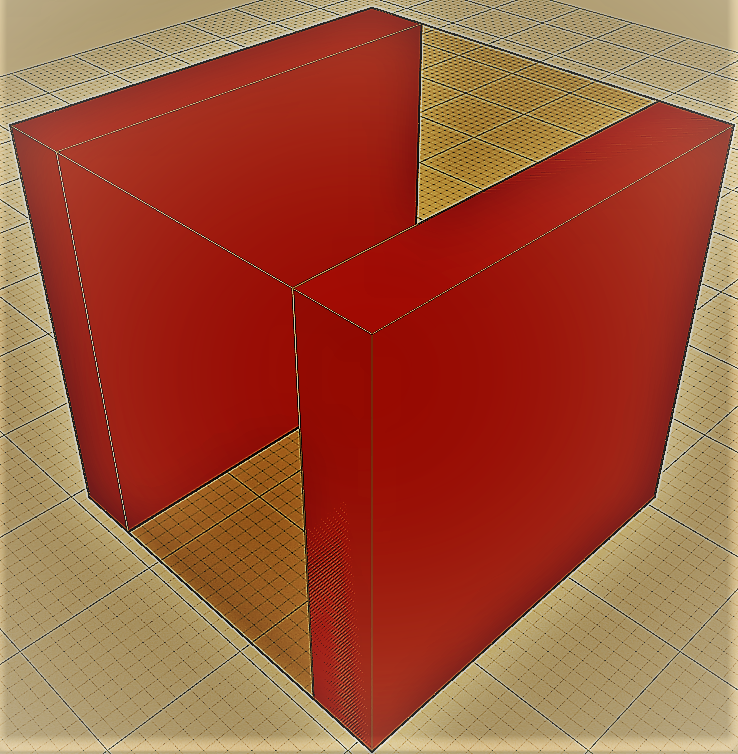
\includegraphics[height=2cm,width=2cm]{3dfractal_1.png}
            \hfill
            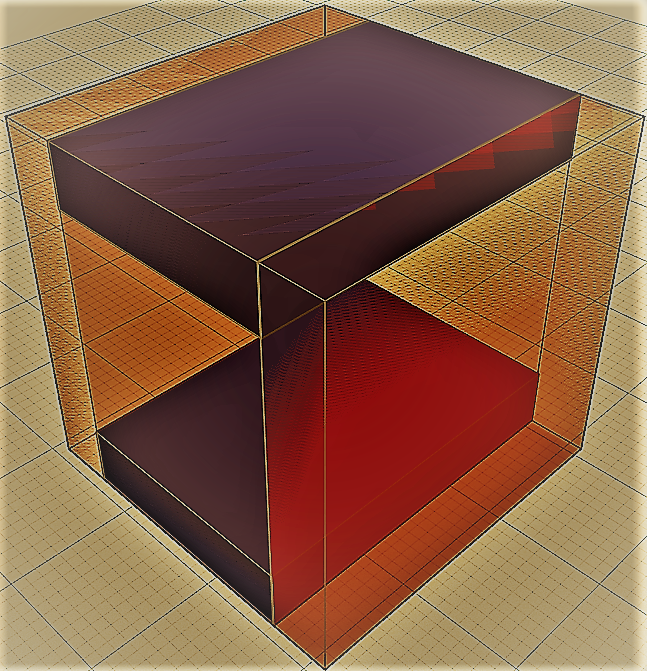
\includegraphics[height=2cm,width=2cm]{3dfractal_2.png}
            \hfill
            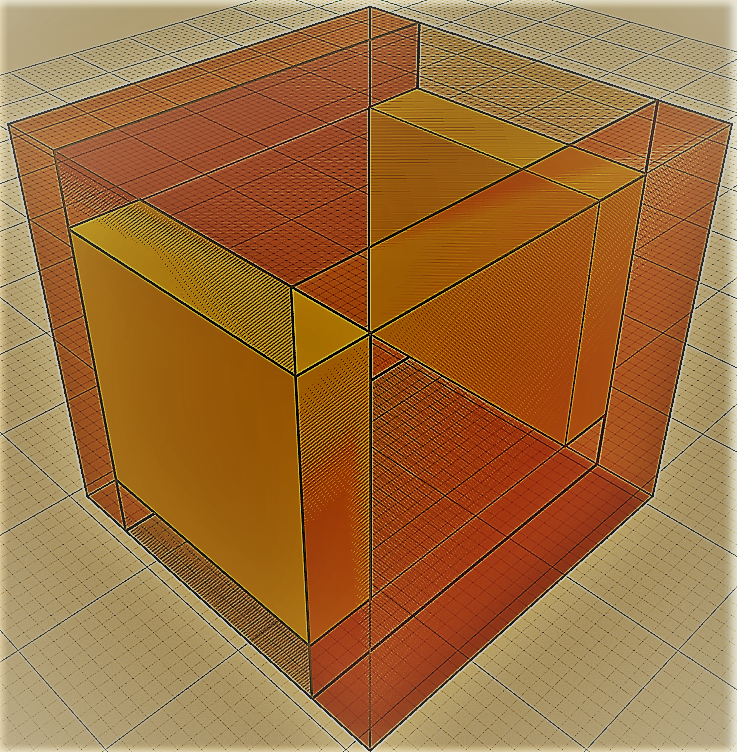
\includegraphics[height=2cm,width=2cm]{3dfractal_3.png}
            \hfill
            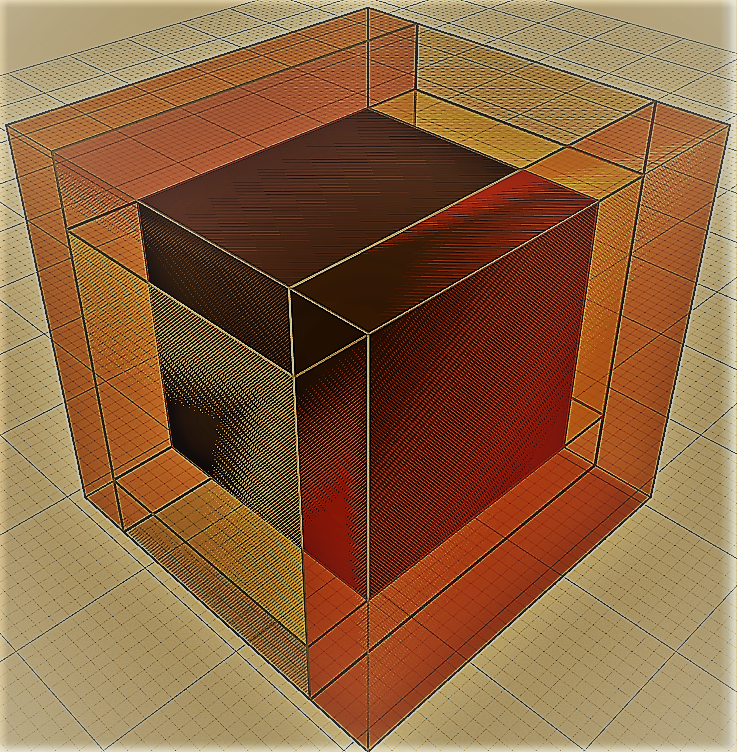
\includegraphics[height=2cm,width=2cm]{3dfractal_4.png}
            \hfill
            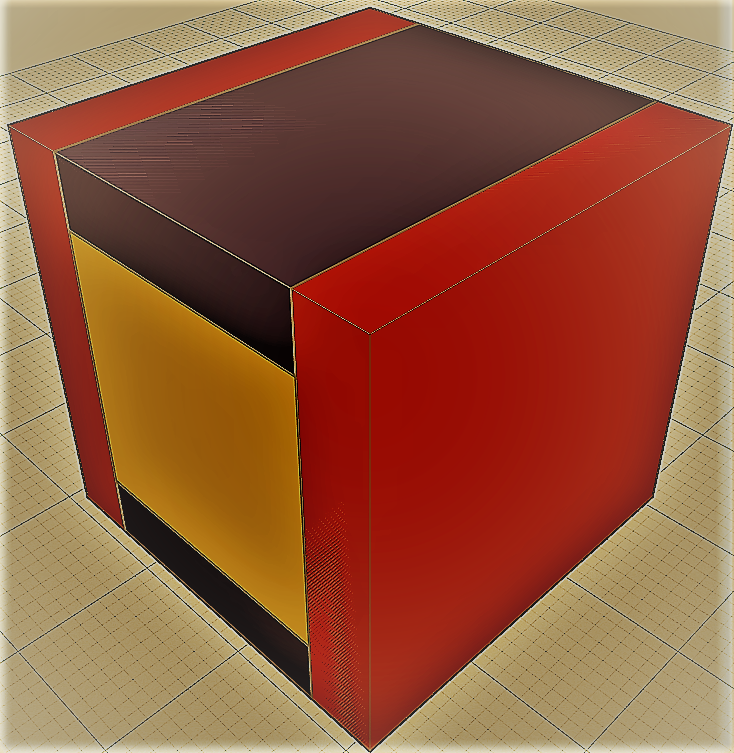
\includegraphics[height=2cm,width=2cm]{3dfractal_5}
        \end{figure}
        
        \begin{align*}
V(\epsilon) &= \textcolor{red}{2\epsilon\cdot N_{\Omega_1}(2\epsilon) \cdot \left( \sum\nolimits_{j=1}^{{N_{\Omega_2}}(2\epsilon)}\p_j \right) \cdot \left( \sum\nolimits_{j=1}^{{N_{\Omega_3}}(2\epsilon)}\q_j \right)} +\\
 &\textcolor{blue}{2\epsilon\cdot N_{\Omega_2}(2\epsilon) \cdot \left( \sum\nolimits_{j=1}^{{N_{\Omega_1}}(2\epsilon)}\ell_j - 2\epsilon \right) \cdot \left( \sum\nolimits_{j=1}^{{N_{\Omega_3}}(2\epsilon)}\q_j \right)} + \\
&\textcolor{orange}{2\epsilon\cdot N_{\Omega_3}(2\epsilon) \cdot \left( \sum\nolimits_{j=1}^{{N_{\Omega_2}}(2\epsilon)}\p_j - 2\epsilon \right) \cdot \left( \sum\nolimits_{j=1}^{{N_{\Omega_1}}(2\epsilon)}\ell_j - 2\epsilon \right)} + \\
&\W_1\SL_2\SL_3 + \SL_1\W_2\SL_3 + \SL_1\SL_2\W_3 - \SL_1\W_2\W_3 - \W_1\SL_2\W_3 - \\
&\W_1\W_2\SL_3 + \W_1\W_2\W_3 
	\end{align*}
	
\end{frame}

\begin{frame}{3 Dimensional Fractal Volume}
$V(\epsilon) = 2\epsilon \cdot N_{\Omega_1}\cdot(\SL_2-\W_3)\cdot(\SL_3-\W_3) + 2\epsilon \cdot N_{\Omega_2}\cdot(\SL_1-\W_1-2\epsilon\cdot N_{\Omega_1})\cdot(\SL_3-\W_3) + 2\epsilon \cdot N_{\Omega_3}\cdot(\SL_2-\W_2-2\epsilon\cdot N_{\Omega_2})\cdot(\SL_1-\W_1-2\epsilon\cdot N_{\Omega_1}) + \W_1\SL_2\SL_3 + \SL_1\W_2\SL_3 + \SL_1\SL_2\W_3 - \SL_1\W_2\W_3 - \W_1\SL_2\W_3 - \W_1\W_2\SL_3 + \W_1\W_2\W_3$

\pause
\vspace{.2in}

$V(\epsilon) = \SL_1\SL_2V_3(\epsilon) + \SL_1V_2(\epsilon)\SL_3 + V_1(\epsilon)\SL_2\SL_3 - V_1(\epsilon)V_2(\epsilon)\SL_3 - V_1(\epsilon)\SL_2V_3(\epsilon)-\SL_1V_2(\epsilon)V_3(\epsilon) + V_1(\epsilon)V_2(\epsilon)V_3(\epsilon)$
\end{frame}

\begin{frame}{4 Dimensional Fractal Objects}
$V(\epsilon) = 2\epsilon\cdot N_{\Omega_1}(2\epsilon) \cdot \left( \sum_{j=1}^{{N_{\Omega_2}}(2\epsilon)}\p_j \right) \cdot \left( \sum_{j=1}^{{N_{\Omega_3}}(2\epsilon)}\q_j \right) \cdot \left( \sum_{j=1}^{{N_{\Omega_4}}(2\epsilon)}\z_j \right) + 2\epsilon\cdot N_{\Omega_2}(2\epsilon) \cdot \left( \sum_{j=1}^{{N_{\Omega_1}}(2\epsilon)}\ell_j - 2\epsilon \right) \cdot \left( \sum_{j=1}^{{N_{\Omega_3}}(2\epsilon)}\q_j \right) \cdot \left( \sum_{j=1}^{{N_{\Omega_4}}(2\epsilon)}\z_j \right) + 2\epsilon\cdot N_{\Omega_3}(2\epsilon) \cdot \left( \sum_{j=1}^{{N_{\Omega_2}}(2\epsilon)}\p_j - 2\epsilon \right) \cdot \left( \sum_{j=1}^{{N_{\Omega_1}}(2\epsilon)}\ell_j - 2\epsilon \right) \cdot \left( \sum_{j=1}^{{N_{\Omega_4}}(2\epsilon)}\z_j \right) + 2\epsilon\cdot N_{\Omega_4}(2\epsilon) \cdot \left( \sum_{j=1}^{{N_{\Omega_2}}(2\epsilon)}\p_j - 2\epsilon \right) \cdot \left( \sum_{j=1}^{{N_{\Omega_1}}(2\epsilon)}\ell_j - 2\epsilon \right) \cdot \left( \sum_{j=1}^{{N_{\Omega_3}}(2\epsilon)}\q_j - 2\epsilon \right) + \W_1\SL_2\SL_3\SL_4 + \SL_1\W_2\SL_3\SL_4 + \SL_1\SL_2\W_3\SL_4 + \SL_1\SL_2\SL_3\W_4 - \SL_1\SL_2\W_3\W_4 - \SL_1\W_2\SL_3\W_4 - \SL_1\W_2\W_3\SL_4 - \W_1\SL_2\SL_3\W_4 - \W_1\SL_2\W_3\SL_4 - \W_1\W_2\SL_3\SL_4 + \SL_1\W_2\W_3\W_4 + \W_1\SL_2\W_3\W_4 + \W_1\W_2\SL_3\W_4 + \W_1\W_2\W_3\SL_4 - \W_1\W_2\W_3\W_4$
\end{frame}

\begin{frame}{4 Dimensional Volume Formula}
$V^4(\epsilon) = \SL_1\SL_2\SL_3V_4(\epsilon) + \SL_1\SL_2V_3(\epsilon)\SL_4 + \SL_1V_2(\epsilon)\SL_3\SL_4 + V_1(\epsilon)\SL_2\SL_3\SL_4 - V_1(\epsilon)V_2(\epsilon)\SL_3\SL_4 - V_1(\epsilon)\SL_2V_3(\epsilon)\SL_4 - V_1(\epsilon)\SL_2\SL_3V_4(\epsilon) - \SL_1V_2(\epsilon)V_3(\epsilon)\SL_4 - \SL_1V_2(\epsilon)\SL_3V_4(\epsilon) - \SL_1\SL_2V_3(\epsilon)V_4(\epsilon) + V_1(\epsilon)V_2(\epsilon)V_3(\epsilon)\SL_4 + V_1(\epsilon)V_2(\epsilon)\SL_3V_4(\epsilon) + V_1(\epsilon)\SL_2V_3(\epsilon)V_4(\epsilon) + \SL_1V_2(\epsilon)V_3(\epsilon)V_4(\epsilon) -  V_1(\epsilon)V_2(\epsilon)V_3(\epsilon)V_4(\epsilon)$

\pause
\vspace{.2in}

$V^3(\epsilon) = \SL_1\SL_2V_3(\epsilon) + \SL_1V_2(\epsilon)\SL_3 + V_1(\epsilon)\SL_2\SL_3 - V_1(\epsilon)V_2(\epsilon)\SL_3 - V_1(\epsilon)\SL_2V_3(\epsilon)-\SL_1V_2(\epsilon)V_3(\epsilon) + V_1(\epsilon)V_2(\epsilon)V_3(\epsilon)$

\vspace{.2in}

$V^2(\epsilon) = \SL_1V_2(\epsilon) + V_1(\epsilon)\SL_2 - V_1(\epsilon)V_2(\epsilon)$

\end{frame}

\begin{frame}{Algebraic Manipulations}
$V^2(\epsilon) = \SL_1V_2(\epsilon) + V_1(\epsilon)\SL_2 - V_1(\epsilon)V_2(\epsilon)$
$$= (-1)\cdot(V_1(\epsilon)-\SL_1)\cdot(V_2(\epsilon)-\SL_2) + \SL_1\SL_2$$

\pause
\vspace{.2in}

$V^3(\epsilon) = \SL_1\SL_2V_3(\epsilon) + \SL_1V_2(\epsilon)\SL_3 + V_1(\epsilon)\SL_2\SL_3 - V_1(\epsilon)V_2(\epsilon)\SL_3 - V_1(\epsilon)\SL_2V_3(\epsilon)-\SL_1V_2(\epsilon)V_3(\epsilon) + V_1(\epsilon)V_2(\epsilon)V_3(\epsilon)$

$$= (-1)^2\cdot(V_1(\epsilon)-\SL_1)\cdot(V_2(\epsilon)-\SL_2)\cdot(V_3(\epsilon)-\SL_3) + \SL_1\SL_2\SL_3$$

\end{frame}

\begin{frame}{Algebraic Manipulations}
$V^4(\epsilon) = \SL_1\SL_2\SL_3V_4(\epsilon) + \SL_1\SL_2V_3(\epsilon)\SL_4 + \SL_1V_2(\epsilon)\SL_3\SL_4 + V_1(\epsilon)\SL_2\SL_3\SL_4 - V_1(\epsilon)V_2(\epsilon)\SL_3\SL_4 - V_1(\epsilon)\SL_2V_3(\epsilon)\SL_4 - V_1(\epsilon)\SL_2\SL_3V_4(\epsilon) - \SL_1V_2(\epsilon)V_3(\epsilon)\SL_4 - \SL_1V_2(\epsilon)\SL_3V_4(\epsilon) - \SL_1\SL_2V_3(\epsilon)V_4(\epsilon) + V_1(\epsilon)V_2(\epsilon)V_3(\epsilon)\SL_4 + V_1(\epsilon)V_2(\epsilon)\SL_3V_4(\epsilon) + V_1(\epsilon)\SL_2V_3(\epsilon)V_4(\epsilon) + \SL_1V_2(\epsilon)V_3(\epsilon)V_4(\epsilon) -  V_1(\epsilon)V_2(\epsilon)V_3(\epsilon)V_4(\epsilon)$
$$ = (-1)^3\cdot(V_1(\epsilon)-\SL_1)\cdot(V_2(\epsilon)-\SL_2)\cdot(V_3(\epsilon)-\SL_3)\cdot(V_4(\epsilon)-\SL_4) + \SL_1\SL_2\SL_3\SL_4$$
\end{frame}

\begin{frame}{General Volume Formula}

$$V^2(\epsilon)= (-1)\cdot(V_1(\epsilon)-\SL_1)\cdot(V_2(\epsilon)-\SL_2) + \SL_1\SL_2$$

$$ V^3(\epsilon) = (-1)^2\cdot(V_1(\epsilon)-\SL_1)\cdot(V_2(\epsilon)-\SL_2)\cdot(V_3(\epsilon)-\SL_3) + \SL_1\SL_2\SL_3$$

$$ V^4(\epsilon)= (-1)^3\cdot(V_1(\epsilon)-\SL_1)\cdot(V_2(\epsilon)-\SL_2)\cdot(V_3(\epsilon)-\SL_3)\cdot(V_4(\epsilon)-\SL_4) + \SL_1\SL_2\SL_3\SL_4$$

$$V^{n}(\epsilon) =\left[ (-1)^{n-1} \cdot \displaystyle \prod_{k = 1}^{n}(V_k(\epsilon)-\SL_k)\right] +\prod_{k = 1}^{n} \SL_k$$

\end{frame}

\end{document}
